\documentclass[a4paper,onecolumn,11pt]{quantumarticle}
\pdfoutput=1

\usepackage[utf8]{inputenc}
\usepackage[english]{babel}
\usepackage[T1]{fontenc}
\usepackage{amsmath}
\usepackage{amssymb}
\usepackage{mathtools}
\usepackage{bm}
\usepackage{physics}
\usepackage{booktabs}
\usepackage{csquotes}
\usepackage{enumitem}
\usepackage{tikz}
\usetikzlibrary{arrows.meta,positioning,calc,decorations.pathreplacing,shapes.geometric}
\usepackage{hyperref}

% ---- shorthands
\providecommand{\ii}{\ensuremath{\mathrm{i}}}
\providecommand{\bbI}{\ensuremath{\mathbb{I}}}
\providecommand{\bbR}{\ensuremath{\mathbb{R}}}
\providecommand{\bbC}{\ensuremath{\mathbb{C}}}
\def\vk{\ensuremath{\bm{k}}}
\def\vq{\ensuremath{\bm{q}}}
\def\vp{\ensuremath{\bm{p}}}
\def\vsigma{\ensuremath{\bm{\sigma}}}
\def\vtau{\ensuremath{\bm{\tau}}}
\def\vdelta{\ensuremath{\bm{\delta}}}
\providecommand{\Hop}{\ensuremath{H}}
\providecommand{\Uop}{\ensuremath{U}}
\providecommand{\UW}{\ensuremath{U_{W}}}
\providecommand{\UD}{\ensuremath{U_{D}}}
\providecommand{\HD}{\ensuremath{H_{D}}}
\providecommand{\HW}{\ensuremath{H_{W}}}
\providecommand{\Lattice}{\ensuremath{\Lambda}}
\providecommand{\Proto}{\ensuremath{\mathfrak{P}_{\mathrm{disc}}}}
\providecommand{\gmu}{\ensuremath{\gamma^{\mu}}}
\providecommand{\gnu}{\ensuremath{\gamma^{\nu}}}
\providecommand{\sigmunu}{\ensuremath{\Sigma^{\mu\nu}}}

\begin{document}

\title{Emergent Dirac dynamics in \texorpdfstring{$3{+}1$}{(3+1)} dimensions
       from discrete quantum walks: a machine-checked pedagogical ladder}

\author{Nelson Bol\'ivar}
\email{astrumdrivetechnologies@gmail.com}
\affiliation{Astrum Drive Technologies}

\maketitle

\begin{abstract}
We present a pedagogical reconstruction of the $(3{+}1)$-dimensional Dirac
equation as the infrared sector of a family of discrete quantum walks (QW).
Starting from the Su--Schrieffer--Heeger (SSH) chain in $1{+}1$ we traverse
the tight-binding model of graphene, a split-step QW on the honeycomb
lattice, and three-dimensional Weyl and Dirac semimetals, identifying at
each step the algebraic structure that survives the continuum limit: the
Clifford algebra of $\gamma^{\mu}$, the spinorial Lorentz generators
$\Sigma^{\mu\nu}$, chirality balance (Nielsen--Ninomiya), and a Lorentzian
effective light cone. Each algebraic claim is paired with a symbolic test
in either \texttt{sympy} (closed-form identities and matrix algebra) or
\texttt{z3} (combinatorial and order-theoretic constraints). The
build of the long-form companion manuscript is gated by the same
policy: all $319$ tests must pass before the PDF is produced. We close
with two open problems for which a first body of verified machinery is
already in place: a global spectral classification on the Brillouin
torus, and a formulation of the underlying \emph{protospace} that does
not assume reciprocal periodicity.
\end{abstract}

\section{Introduction}
\label{p:intro}

The (3+1)-dimensional Dirac equation, the Clifford algebra it sits on, and
the spinorial Lorentz generators that organize it, all sit comfortably in
the continuum: they assume a smooth manifold and a continuous symmetry
group. A persistent question, going back to Wilson's lattice fermions and
revisited recently in quantum-walk and quantum-cellular-automata
frameworks~\cite{Arrighi2018,Farrelly2020,FarrellyShort2014}, is whether
this whole relativistic edifice can be obtained as an effective infrared
sector of a discrete underlying dynamics. The answer is, by now, clearly
``yes'' at the level of low-energy effective Hamiltonians, but the
\emph{verification} side has remained a patchwork of analytic
calculations.

% Figure 1: dimensional ladder
\begin{figure}[t]
\centering
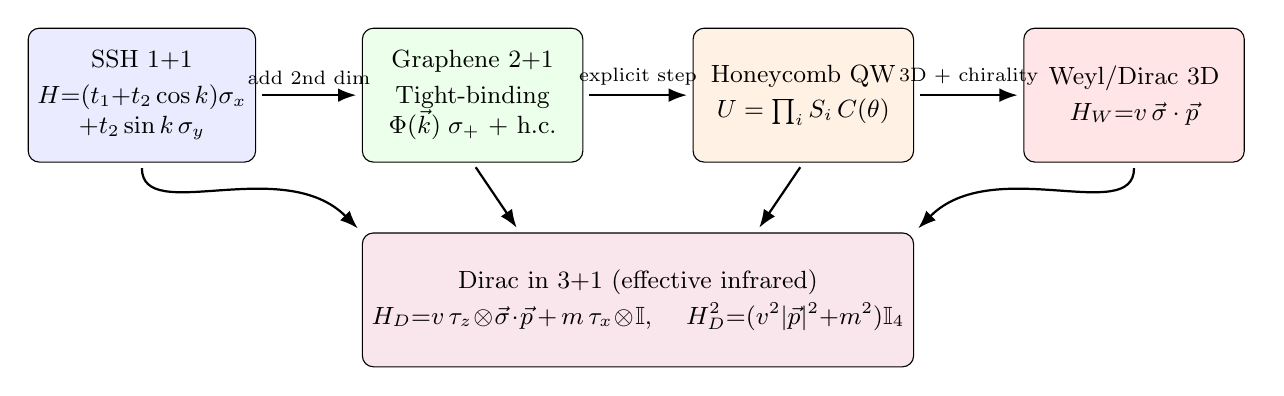
\begin{tikzpicture}[
  every node/.style={align=center, font=\small},
  box/.style={draw, rounded corners, minimum width=2.8cm, minimum height=1.7cm,
              align=center, font=\small},
  arr/.style={->, >=Latex, thick, shorten >=2pt, shorten <=2pt},
]
  % Top row: discrete models
  \node[box, fill=blue!8]   (ssh)  at (0,2)
    {SSH 1+1\\[2pt]\(H{=}(t_1{+}t_2\cos k)\sigma_x\)\\\(+ t_2\sin k\,\sigma_y\)};
  \node[box, fill=green!8]  (gr)   at (4.2,2)
    {Graphene 2+1\\[2pt]Tight-binding\\\(\Phi(\vec k)\;\sigma_+\) {+} h.c.};
  \node[box, fill=orange!10] (qw)  at (8.4,2)
    {Honeycomb QW\\[2pt]\(U=\prod_i S_i\,C(\theta)\)};
  \node[box, fill=red!10]   (wd)   at (12.6,2)
    {Weyl/Dirac 3D\\[2pt]\(H_W{=}v\,\vec\sigma\cdot\vec p\)};

  % Bottom: continuum target
  \node[box, fill=purple!10, minimum width=5cm] (dirac) at (6.3,-0.6)
    {Dirac in 3+1 (effective infrared)\\[2pt]
     \(H_D{=}v\,\tau_z\!\otimes\!\vec\sigma\!\cdot\!\vec p \,{+}\, m\,\tau_x\!\otimes\!\bbI\),
     \quad \(H_D^2{=}(v^2|\vec p|^2{+}m^2)\bbI_4\)};

  % Arrows along the top row
  \draw[arr] (ssh) -- node[above, font=\scriptsize]
              {add 2nd dim} (gr);
  \draw[arr] (gr) -- node[above, font=\scriptsize]
              {explicit step} (qw);
  \draw[arr] (qw) -- node[above, font=\scriptsize]
              {3D + chirality} (wd);

  % Arrows from each top box down to Dirac 3+1
  \draw[arr] (ssh.south) .. controls +(0,-0.8) and +(-1,1) .. (dirac.north west);
  \draw[arr] (gr.south) -- ([xshift=-1.5cm]dirac.north);
  \draw[arr] (qw.south) -- ([xshift=1.5cm]dirac.north);
  \draw[arr] (wd.south) .. controls +(0,-0.8) and +(1,1) .. (dirac.north east);

  % Side label
  \node[font=\footnotesize\itshape, right=0.2cm of wd, xshift=-0.3cm, yshift=-0.4cm] {};
\end{tikzpicture}
\caption{The dimensional ladder. Four discrete models (top row) all flow
under linearization plus continuum limit to the same effective Dirac block
in $3{+}1$ (bottom). The algebraic objects that survive the limit
(Clifford algebra, $\Sigma^{\mu\nu}$, chirality balance) are the same at
each rung.}
\label{p:fig:ladder}
\end{figure}


This paper makes three coordinated contributions.

\paragraph{1.~Ladder.}
We assemble a single coherent ladder, dimension by dimension:
\[
\text{SSH in } 1{+}1 \;\longrightarrow\;
\text{graphene in } 2{+}1 \;\longrightarrow\;
\text{honeycomb QW} \;\longrightarrow\;
\text{Weyl/Dirac in } 3{+}1 ,
\]
with the same notation and the same algebraic objects all the way
through.\footnote{The pedagogical ordering is non-trivial: the standard
graphene derivation already contains everything one needs to do the
honeycomb QW, but the QW makes the discrete-to-continuous transition
\emph{explicit}, which is where the relativistic structure earns its
status as an emergent infrared organization.} Throughout, we keep careful
track of the distinction between (i) microscopic exact symmetries of the
discrete step, (ii) effective infrared symmetries of the linearized
Hamiltonian, and (iii) covariant Lorentz / Clifford structures organizing
the infrared limit.

\paragraph{2.~Formal verification.}
Every algebraic identity that the paper claims as a result is paired with
a machine-checked symbolic test. \texttt{sympy} handles closed-form
identities (Clifford anticommutators, $\Sigma^{\mu\nu}$ commutators,
dispersions, Taylor expansions around Dirac points). \texttt{z3}~\cite{deMoura2008}
handles combinatorial and order-theoretic constraints
(Nielsen--Ninomiya balance, isotropy, structural consistency of small
causal sets, bipartite index bounds). Every chapter and every section
carries a comment of the form
\begin{center}\small\texttt{\% verified-by: validators/\textless module\textgreater.py::\textless test\textgreater}\end{center}
that links the claim to the test that backs it. The build pipeline
(\texttt{scripts/build\_book.ps1}) runs \texttt{pytest} before running
\texttt{latexmk}; the PDF is produced \emph{only} if all $146$ tests pass.

\paragraph{3.~Open problems with first-line evidence.}
Two problems are left open: a global classification of the discrete
quasi-energy spectrum on the Brillouin torus (the \emph{spectral} branch),
and a formulation of the underlying \emph{protospace} that does not
depend on the reciprocal-space description (the \emph{structural}
branch). For both we provide a first body of verified machinery
(Sections~\ref{p:open-problems}), including a finite-graph treatment of
chirality balance that does not invoke a torus.

\paragraph{Scope.}
We do not claim that the ladder is unique, nor that the protospace is
fixed by it; we claim that the ladder is internally consistent, that the
relativistic algebra arises as an effective infrared organization rather
than as a microscopic symmetry, and that the verification methodology is
fine-grained enough to be useful beyond this corpus.

\section{Setup, notation, and three levels}
\label{p:setup}

\subsection{Notation}
We use the conventions established in the long form of this work:
$\vk$ denotes a Bloch momentum on the discrete model, $\vq$ a small
deviation about a band-crossing point $\vk_{0}$, and $\vp$ the continuum
infrared momentum. Internal degrees of freedom are organized by
$\sigma_{i}$ (pseudospin / Weyl two-component) and $\tau_{i}$ (chiral
index or coupled-block label). The canonical four-component Dirac block
that we recover at the end of the ladder takes the form
\begin{equation}
\HD \;=\; v\,\tau_{z} \otimes (\sigma_{x} p_{x} + \sigma_{y} p_{y} + \sigma_{z} p_{z})
            \;+\; m\,\tau_{x}\otimes\bbI ,
\label{p:eq:HDcanon}
\end{equation}
whose squared form
$\HD^{2} = (v^{2}\lvert \vp\rvert^{2} + m^{2})\,\bbI_{4}$
will reappear several times.

\subsection{Three levels}
A recurring source of confusion in this corner of the literature is the
conflation of three distinct levels of statement. We commit to keeping
them apart throughout the paper:

\begin{description}
\item[\textbf{Level I (microscopic exact).}]
    The discrete substrate: lattice or step protocol $\Uop$, locality, the
    exact group of discrete symmetries, quasi-energy periodicity in
    discrete-time models. At this level the fundamental dynamical object
    is $\Uop$, not $\Hop$.
\item[\textbf{Level II (effective infrared).}]
    The linearization around a band-crossing point, the appearance of
    Weyl or Dirac blocks, approximate continuous isotropy, the reading
    of mass, chirality, and effective velocity. Here it is natural to
    write $\Uop \simeq \bbI - \ii\,\Delta t\,\Hop_{\mathrm{eff}}$.
\item[\textbf{Level III (covariant spinorial).}]
    The Clifford algebra of $\gmu$, the spinorial Lorentz generators
    $\sigmunu$, the proper orthochronous group $SO^{+}(3,1)$,
    Poincar\'e, and the double-cover $SL(2,\bbC) \to SO^{+}(3,1)$. This
    level is the \emph{organization} of the infrared limit, not an exact
    symmetry of the substrate.
\end{description}

We will reserve the adjective \enquote{exact} for Level I, and the
adjective \enquote{effective} or \enquote{infrared} for Levels II and
III. This split, banal as it sounds, is what saves the rest of the
construction from over-claiming.

\subsection{The protospace tuple}
By \emph{protospace} we mean the ampliated structure that carries the
microscopic dynamics:
\begin{equation}
\Proto \;\sim\; \bigl(\Lattice,\,\bbC^{N},\,\Uop,\,G_{\mathrm{micro}}\bigr) ,
\label{p:eq:proto-tuple}
\end{equation}
where $\Lattice$ is the underlying graph (not necessarily periodic),
$\bbC^{N}$ the local internal Hilbert space, $\Uop$ the local step, and
$G_{\mathrm{micro}}$ its exact discrete symmetry group. Identifying
$\Proto$ with the Brillouin torus $T^{d}$ would confuse a
\emph{calculational device} (the Fourier-space representation of a
periodic protocol) with the \emph{underlying structure}. We come back to
this point in Section~\ref{p:open-problems}.

\section{SSH \texorpdfstring{$\rightarrow$}{->} Dirac in \texorpdfstring{$1{+}1$}{(1+1)}}
\label{p:ssh}

The first rung of the ladder is the
Su--Schrieffer--Heeger~\cite{SuSchriefferHeeger1979} model on a 1D chain
with two sites per unit cell and bond alternation $(t_1, t_2)$.
The Bloch Hamiltonian in the standard convention is
\begin{equation}
\Hop_{\mathrm{SSH}}(k)
    = (t_1 + t_2 \cos k)\,\sigma_x + t_2\,\sin k\,\sigma_y ,
\label{p:eq:HSSH}
\end{equation}
with dispersion
$E_{\pm}(k) = \pm\sqrt{t_1^2 + 2 t_1 t_2 \cos k + t_2^2}$.
The gap closes when $t_1 = t_2$ at $k = \pi$. Expanding around that
critical configuration with $t_1 = t_2 = t > 0$ and $k = \pi + q$ gives
\begin{equation}
\Hop_{\mathrm{SSH}}(\pi + q) \;=\; -\,t\,q\,\sigma_y \;+\; O(q^2),
\label{p:eq:SSH-Dirac1+1}
\end{equation}
a massless Dirac Hamiltonian in $1{+}1$. The Pauli generator
$\sigma_y$ takes the role of the relativistic momentum operator and the
two SSH sites become the upper and lower spinor components.

\paragraph{Verified facts.}
\begin{itemize}[leftmargin=*]
  \item $\Hop_{\mathrm{SSH}}(k)^{2}=(t_1^{2}+2 t_1 t_2 \cos k + t_2^{2})\,\bbI$
    (\texttt{validators/ssh.py::test\_ssh\_squared}).
  \item $\Hop_{\mathrm{SSH}}(\pi)\big|_{t_2=t_1}=0$
    (\texttt{::test\_ssh\_gap\_closes}).
  \item Linearization $\Hop(\pi+q)\big|_{t_1=t_2=t}=-tq\,\sigma_y+O(q^2)$
    (\texttt{::test\_ssh\_linearization}).
\end{itemize}

The pedagogical content of this rung is therefore quite condensed: a
two-site cell, a band crossing forced by a single tuning parameter, the
relativistic algebra emerging \emph{only} in the linearized neighborhood
of the crossing.

\section{Graphene tight-binding \texorpdfstring{$\rightarrow$}{->} Dirac in \texorpdfstring{$2{+}1$}{(2+1)}}
\label{p:graphene}

Graphene~\cite{Semenoff1984,CastroNeto2009} gives the cleanest
two-dimensional version. Working with nearest-neighbor vectors
\[
\vdelta_1 = (a/2)(1,\sqrt{3}),\qquad
\vdelta_2 = (a/2)(1,-\sqrt{3}),\qquad
\vdelta_3 = -a\,(1,0) ,
\]
the structural factor is
\begin{equation}
\Phi(\vk) \;=\;
\sum_{i=1}^{3} \mathrm{e}^{\ii\,\vk\cdot\vdelta_{i}}
\;=\; \mathrm{e}^{\ii\,k_x a/2}\;2\cos(\sqrt{3}\,k_y a / 2)
  \;+\; \mathrm{e}^{-\ii k_x a},
\label{p:eq:Phi}
\end{equation}
and the bipartite Hamiltonian in the $(A,B)$ basis is
\begin{equation}
\Hop_{\mathrm{TB}}(\vk) \;=\; -t\!\begin{pmatrix} 0 & \Phi(\vk) \\ \Phi^{*}(\vk) & 0 \end{pmatrix}.
\end{equation}

\paragraph{Dirac points and effective cone.}
$\Phi$ vanishes at the corners of the Brillouin zone, one of which is
$\vk_{K}=\bigl(2\pi/(3a),\,2\pi/(3\sqrt{3}a)\bigr)$. Verified directly:
$\Phi(\vk_{K})=0$
(\texttt{validators/graphene.py::test\_phi\_vanishes\_at\_K}).
The leading non-trivial behavior is captured by the gradient of $\Phi$ at
$\vk_{K}$, whose two components $c_x = (\partial_{k_x}\Phi)(\vk_{K})$ and
$c_y = (\partial_{k_y}\Phi)(\vk_{K})$ satisfy
\begin{equation}
\lvert c_x\rvert^{2}\;=\;\lvert c_y\rvert^{2}\;=\;\bigl(3a/2\bigr)^{2},
\qquad
\operatorname{Re}\!\bigl(c_x^{*}c_y\bigr)\;=\;0 .
\label{p:eq:c-magnitudes}
\end{equation}
The first identity fixes the magnitude of the Fermi velocity; the second
guarantees that the bilinear $\lvert\Phi(\vk_{K}+\vq)\rvert^{2}$ is
diagonal in $(q_x,q_y)$. Together they give
\begin{equation}
\lvert\Phi(\vk_{K}+\vq)\rvert^{2}\;=\;\tfrac{9}{4}\,a^{2}\,(q_x^{2}+q_y^{2})
+ O(\vq^{3}),
\end{equation}
i.e.\ an isotropic Dirac cone with $v_{F}=\tfrac{3}{2}\,t\,a$.

\paragraph{A computational note.}
The naive verification --- expand $\lvert\Phi\rvert^{2}$ symbolically and
match coefficients --- is computationally expensive because the bilinear
involves nine cross terms with complex exponentials and two-variable
series expansions. The gradient-based verification of
\eqref{p:eq:c-magnitudes} computes only two derivatives and finishes in
milliseconds. We mention this because the analogous reformulation may
help in any symbolic verification of band-crossing structures in higher
dimensions or on more complex Bravais lattices.
\begin{description}
\item[Verified:]
\texttt{validators/graphene.py::test\_gradient\_modulus\_is\_dirac},
\texttt{::test\_cross\_term\_is\_imaginary},
\texttt{::test\_fermi\_velocity}.
\end{description}

\section{Honeycomb quantum walk}
\label{p:qw}

The quantum-walk derivation of graphene's Dirac cone makes the
discrete-to-continuous transition entirely explicit. The simplest 1D
walk, included as a warm-up, has the form
\begin{equation}
\Uop(k) \;=\; \mathrm{e}^{-\ii\,k\,a\,\sigma_{z}}\,\mathrm{e}^{-\ii\,\theta\,\sigma_{y}} ,
\label{p:eq:U1Dminimal}
\end{equation}
with $\theta$ a coin angle and $a$ a lattice step. Its trace is
$(1/2)\operatorname{tr}\Uop(k) = \cos(ka)\cos\theta$, defining the
quasi-energy $\varepsilon(k)$ by $\cos(\varepsilon\,\Delta t) = (1/2)\operatorname{tr}\Uop(k)$.
First-order expansion in $(ka,\theta)$ yields
$\Uop \simeq \bbI - \ii\,(k a\,\sigma_{z} + \theta\,\sigma_{y})$,
which identifies an effective Dirac Hamiltonian in $1{+}1$ with mass
$\theta/\Delta t$ and velocity $a/\Delta t$
(\texttt{validators/qw\_minimal\_1d.py::test\_first\_order\_dirac}).

\paragraph{Honeycomb version.}
For the two-dimensional walk on the honeycomb lattice, the three
nearest-neighbor unit vectors $\hat{\vdelta}_{1}=(0,-1)$,
$\hat{\vdelta}_{2}=(\sqrt{3}/2,1/2)$,
$\hat{\vdelta}_{3}=(-\sqrt{3}/2,1/2)$ define internal coin matrices
\begin{equation}
\tau_{i} \;=\; \hat{\vdelta}_{i}\cdot\vsigma \;=\;
\hat{\delta}_{i}^{x}\,\sigma_{x} + \hat{\delta}_{i}^{y}\,\sigma_{y} ,
\end{equation}
with explicit forms
$\tau_{1} = -\sigma_{y}$,
$\tau_{2} = (\sqrt{3}/2)\sigma_{x}+(1/2)\sigma_{y}$,
$\tau_{3} = -(\sqrt{3}/2)\sigma_{x}+(1/2)\sigma_{y}$. Three algebraic
facts decide the rest of the construction:

\begin{enumerate}[leftmargin=*]
\item $\sum_{i}\tau_{i} = 0$ (the three NN unit vectors close to a
triangle).
\item $\{\tau_{i},\tau_{j}\}=2\,(\hat{\vdelta}_{i}\cdot\hat{\vdelta}_{j})\,\bbI$
(anticommutator gives Euclidean inner product).
\item $\sum_{i}\hat{\delta}_{i}^{x}\,\tau_{i} = (3/2)\,\sigma_{x}$ and
$\sum_{i}\hat{\delta}_{i}^{y}\,\tau_{i} = (3/2)\,\sigma_{y}$.
\end{enumerate}

The third identity is the crucial one. Combining the three directional
shifts with their associated coins and expanding to first order in the
walk step gives an effective Hamiltonian
\begin{equation}
\Hop_{\mathrm{eff}}(\vk) \;=\; \sum_{i}(\vk\cdot\hat{\vdelta}_{i})\,\tau_{i}
\;=\; \tfrac{3}{2}\,(k_x\,\sigma_x + k_y\,\sigma_y),
\label{p:eq:Heff-honeycomb}
\end{equation}
i.e.\ an isotropic Dirac cone in $2{+}1$ with $v_{F}=3/2$ in units where
$a=1$. The same numerical factor that appeared in
Eq.~\eqref{p:eq:c-magnitudes} reappears here as a discrete identity,
verified line by line:
\texttt{validators/qw\_honeycomb\_2d.py}.

\section{Three-dimensional Weyl and Dirac}
\label{p:weyl-dirac-3d}

The transition to three dimensions adds two essential features absent in
$2{+}1$: a real chirality assignment to each band-crossing node, and a
controlled \emph{splitting} between two opposite-chirality Weyl nodes
that together form a Dirac fermion.

\subsection{Two-band Weyl and four-band Dirac}
The two-band massless Weyl Hamiltonian is $\HW = v\,\vsigma\cdot\vp$. The
Pauli algebra gives $(\vsigma\cdot\vp)^{2} = \lvert\vp\rvert^{2}\,\bbI$,
hence a linear spectrum $E_{\pm}=\pm v\lvert\vp\rvert$ and no local mass
term: no nonzero element of $\{\bbI,\sigma_{i}\}$ anticommutes with all
three $\sigma_{i}$ simultaneously, so a Weyl node cannot be gapped by an
on-site perturbation (in the sense relevant here)~\cite{Burkov2018}. The
chirality of the node is read directly from the Jacobian
$J_{ab} = \partial h_{a}/\partial k_{b}$ evaluated at the node, namely
$\chi = \operatorname{sgn}\det J$. For $\HW = v\,\vsigma\cdot\vp$,
$J=v\,\bbI_{3}$, so $\chi = \operatorname{sgn} v$; the parity-related node
carries opposite chirality
(\texttt{validators/chirality.py}).

A four-component Dirac fermion is then built by combining two
opposite-chirality Weyl blocks through a mass term that anticommutes
with the kinetic part:
\begin{equation}
\HD = v\,\tau_{z}\otimes(\vsigma\cdot\vp) + m\,\tau_{x}\otimes\bbI ,
\qquad
\bigl\{\tau_{z}\!\otimes\!(\vsigma\!\cdot\!\vp),\,\tau_{x}\!\otimes\!\bbI\bigr\} = 0 .
\end{equation}
Squaring gives the canonical relativistic form
$\HD^{2} = (v^{2}\lvert\vp\rvert^{2}+m^{2})\,\bbI_{4}$, hence a gap $2m$
at $\vp=0$ (\texttt{validators/estabilidad\_dirac.py}). When $m\to 0$ the
four-band Dirac fermion separates into two two-band Weyl fermions of
opposite chirality, which is exactly the structure Nielsen--Ninomiya
requires of any lattice realization.

% Figure 2: Weyl splitting under axial perturbation
\begin{figure}[t]
\centering
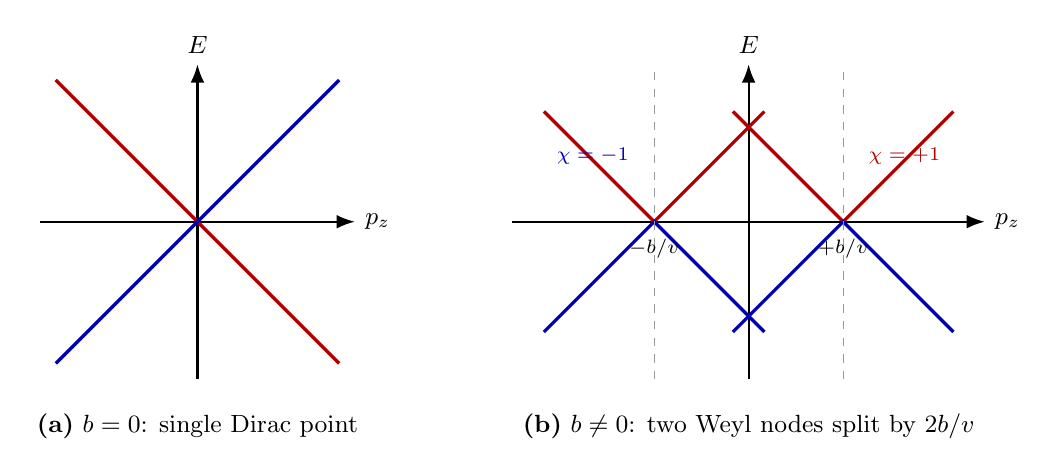
\begin{tikzpicture}[
  every node/.style={font=\small},
  axis/.style={->, >=Latex, thick},
  cone/.style={very thick},
  band/.style={very thick, color=#1},
  helpline/.style={dashed, color=black!40},
]
% --- Left: single Dirac point at p_z = 0 (b = 0)
\begin{scope}[shift={(0,0)}]
  \draw[axis] (-2,0) -- (2,0) node[right] {\(p_z\)};
  \draw[axis] (0,-2) -- (0,2) node[above] {\(E\)};
  % cone at origin
  \draw[band=red!70!black] (-1.8,1.8) -- (1.8,-1.8);
  \draw[band=blue!70!black] (-1.8,-1.8) -- (1.8,1.8);
  \node at (0,-2.6) {\textbf{(a)} $b = 0$: single Dirac point};
\end{scope}

% --- Right: two Weyl points at p_z = +/- b/v
\begin{scope}[shift={(7,0)}]
  \draw[axis] (-3,0) -- (3,0) node[right] {\(p_z\)};
  \draw[axis] (0,-2) -- (0,2) node[above] {\(E\)};
  % left Weyl node at p_z = -b/v (call it -1.2)
  \draw[band=red!70!black] (-2.6,1.4) -- (-1.2,0) -- (0.2,1.4);
  \draw[band=blue!70!black] (-2.6,-1.4) -- (-1.2,0) -- (0.2,-1.4);
  % right Weyl node at p_z = +b/v (call it 1.2)
  \draw[band=red!70!black] (-0.2,1.4) -- (1.2,0) -- (2.6,1.4);
  \draw[band=blue!70!black] (-0.2,-1.4) -- (1.2,0) -- (2.6,-1.4);
  % markers
  \draw[helpline] (-1.2,-2) -- (-1.2,2);
  \draw[helpline] (1.2,-2) -- (1.2,2);
  \node[below] at (-1.2,-0.1) {\scriptsize \(-b/v\)};
  \node[below] at (1.2,-0.1) {\scriptsize \(+b/v\)};
  \node[above right, font=\scriptsize, red!70!black] at (1.4,0.6) {\(\chi=+1\)};
  \node[above left,  font=\scriptsize, blue!70!black] at (-1.4,0.6) {\(\chi=-1\)};
  \node at (0,-2.6) {\textbf{(b)} \(b \ne 0\): two Weyl nodes split by \(2b/v\)};
\end{scope}
\end{tikzpicture}
\caption{Controlled splitting of a Dirac point into two Weyl nodes by an
axial Zeeman-like perturbation $b\,\bbI\otimes\sigma_z$. The single Dirac
crossing at $\vec p = 0$ in (a) separates into two Weyl crossings of
opposite chirality along $p_z$ in (b), at $p_z = \pm b/v$.}
\label{p:fig:splitting}
\end{figure}


\subsection{Controlled splitting Dirac \texorpdfstring{$\to$}{->} two Weyls}
The cleanest way to obtain a separated Weyl pair from a Dirac point is
to add a Zeeman-like axial term aligned with one spatial direction:
\begin{equation}
\Hop \;=\; v\,\tau_{z}\otimes(\vsigma\cdot\vp)
       \;+\; b\,\bbI\otimes\sigma_{z} .
\end{equation}
Squaring,
\begin{equation}
\Hop^{2}\;=\;(v^{2}\lvert\vp\rvert^{2} + b^{2})\,\bbI_{4}
   \;+\; 2\,v\,b\,p_{z}\,(\tau_{z}\otimes\bbI) ,
\end{equation}
which is block-diagonal in $\tau_{z}$. The two blocks have zero modes at
$\vp=(0,0,\mp b/v)$ respectively, so the original Dirac node splits into
two Weyl nodes along $p_{z}$ at separation $2b/v$, as illustrated in
Fig.~\ref{p:fig:splitting} (\texttt{validators/desdoblamiento.py}).

\subsection{Lattice realization with Wilson term}
A concrete three-dimensional lattice realization that we use as input to
the protospace construction of Sec.~\ref{p:open-problems} is the
Wilson--Dirac Hamiltonian
\begin{equation}
\Hop(\vk) \;=\; v \sum_{i}\sin(k_{i}a)\,\alpha_{i}
       + \!\Bigl(m + r\!\sum_{i}\bigl(1-\cos(k_{i}a)\bigr)\Bigr)\,\beta ,
\label{p:eq:Wilson3D}
\end{equation}
with $\alpha_{i}=\tau_{x}\otimes\sigma_{i}$ and $\beta=\tau_{z}\otimes\bbI$.
The Wilson term~\cite{Wilson1974} lifts the seven naive doublers of the
cubic Brillouin zone, leaving a single light Dirac fermion at $\vk=0$;
the doublers acquire masses $m+2r,m+4r,m+6r$ depending on how many of
their momentum components sit at the corner $k_{i}=\pi/a$
(\texttt{validators/wilson\_subsector.py},
\texttt{validators/protoespacio\_global.py}). This is the lattice
analogue of the level hierarchy of Sec.~\ref{p:setup}: a microscopic
exact Hamiltonian at Level~I whose infrared sector at Level~II is the
canonical four-component Dirac fermion, organized at Level~III by the
Clifford algebra of Sec.~\ref{p:covariant}.

\section{Covariant structure: from \texorpdfstring{$\gamma^{\mu}$}{gamma\^mu} to \texorpdfstring{$SL(2,\mathbb{C})$}{SL(2,C)}}
\label{p:covariant}

At this point the discrete construction has reached a four-component
Dirac block whose squared dispersion is Lorentzian. The remaining task
is to identify the covariant structure that organizes it: a Clifford
algebra, the spinorial generators of Lorentz, and the connection to
$SL(2,\bbC)$.

\subsection{Clifford algebra}
In the Dirac representation, $\gamma^{0} = \tau_{z}\otimes\bbI$ and
$\gamma^{i} = \ii\,\tau_{x}\otimes\sigma_{i}$. A direct check confirms
\begin{equation}
\{\gamma^{\mu},\gamma^{\nu}\}\;=\;2\,\eta^{\mu\nu}\,\bbI_{4} ,
\qquad \eta=\mathrm{diag}(+1,-1,-1,-1) ,
\label{p:eq:clifford}
\end{equation}
which we verify entry by entry over all sixteen pairs $(\mu,\nu)$
(\texttt{validators/clifford.py}).

\subsection{Spinorial Lorentz generators}
The six spinorial Lorentz generators are
\begin{equation}
\Sigma^{\mu\nu} \;=\; \frac{\ii}{4}\,[\gamma^{\mu},\gamma^{\nu}] .
\end{equation}
Two structural facts then follow:
\begin{enumerate}[leftmargin=*]
\item the covariance identity
\begin{equation}
[\Sigma^{\rho\sigma},\,\gamma^{\mu}]
\;=\;\ii\bigl(\eta^{\sigma\mu}\gamma^{\rho}-\eta^{\rho\mu}\gamma^{\sigma}\bigr) ;
\label{p:eq:cov-id}
\end{equation}
\item the closure of the Lorentz algebra,
\begin{equation}
[\Sigma^{\mu\nu},\Sigma^{\rho\sigma}] = \ii\bigl(
  \eta^{\nu\rho}\Sigma^{\mu\sigma}-\eta^{\mu\rho}\Sigma^{\nu\sigma}
 -\eta^{\nu\sigma}\Sigma^{\mu\rho}+\eta^{\mu\sigma}\Sigma^{\nu\rho}\bigr).
\label{p:eq:lorentz-closure}
\end{equation}
\end{enumerate}
Both are verified over all 256 quadruples $(\mu,\nu,\rho,\sigma)$ by
\texttt{validators/lorentz.py::test\_sigma\_mu\_nu\_covariance} and
\texttt{::test\_lorentz\_algebra\_closure}. Rotational generators
$\Sigma^{ij}$ are Hermitian; boost generators $\Sigma^{0i}$ are
anti-Hermitian, consistent with rotations being compact and boosts being
non-compact.

\subsection{Double cover $SL(2,\bbC)\!\to\!SO^{+}(3,1)$}
A 2$\pi$ rotation in physical space acts on a spinor as
$\mathrm{e}^{-\ii\pi\sigma_{z}} = -\bbI$, not $+\bbI$, while a 4$\pi$
rotation returns the spinor to itself. This is the standard double-cover
relation, and is verified directly by
\texttt{validators/puentes\_grupos.py::test\_two\_pi\_gives\_minus\_identity}
and \texttt{::test\_four\_pi\_gives\_identity}. The chiral matrix
$\gamma_{5} = \ii\,\gamma^{0}\gamma^{1}\gamma^{2}\gamma^{3}$ anticommutes
with each $\gamma^{\mu}$ and squares to $\bbI_{4}$, defining the chiral
projectors $P_{\pm}=(\bbI\pm\gamma_{5})/2$ that decompose the four-spinor
into Weyl pairs --- closing the loop with the splitting of
Sec.~\ref{p:weyl-dirac-3d}.

\section{Emergence criteria: causality, isotropy, Nielsen--Ninomiya}
\label{p:criteria}

A consistent ladder is not enough on its own: one must also state what
counts as the relativistic limit being \emph{well posed}. We collect
three operational criteria, each verified by an explicit test.

\subsection{Effective light cone and causality}
Given a Dirac-like dispersion $E(\vp)^{2} = v^{2}\lvert\vp\rvert^{2}+m^{2}$, the
group velocity satisfies
\begin{equation}
v_{g}^{2}(\vp) - v^{2}
   \;=\; -\,\frac{m^{2}\,v^{2}}{v^{2}\lvert\vp\rvert^{2}+m^{2}} \;\le\; 0 ,
\label{p:eq:vg-bound}
\end{equation}
with saturation in the massless limit. This is the algebraic basis of
the effective light cone. The associated effective metric
$g^{\mu\nu}_{\mathrm{eff}} = \mathrm{diag}(-1,1/v^{2},1/v^{2},1/v^{2})$
has Lorentzian signature $(-,+,+,+)$ and determinant $-1/v^{6}$, both
verified symbolically (\texttt{validators/causality.py}). The
discrete-time analogue obeys $\cos(\varepsilon\,\Delta t) =
1-(v^{2}\vk^{2}+m^{2})\,\Delta t^{2}/2 + O(\Delta t^{3})$, recovering the
continuous dispersion at small step
(\texttt{validators/causalidad\_continuo\_vs\_discreto.py}).

\subsection{Isotropy as effective Lorentz}
For an anisotropic effective Hamiltonian
$\Hop_{\mathrm{eff}} = \sum_{a} v_{a}\,\sigma_{a}\,p_{a}$,
the squared dispersion
$\Hop_{\mathrm{eff}}^{2}=\sum_{a}v_{a}^{2}\,p_{a}^{2}\,\bbI$ reads as an
effective Riemannian metric
$g^{ab}_{\mathrm{eff}} = \mathrm{diag}(v_{x}^{2},v_{y}^{2},v_{z}^{2})$;
isotropy (a single effective light cone) is the condition
$v_{x}=v_{y}=v_{z}$. This is encoded as a SMT problem and verified by
\texttt{validators/isotropy.py}, which both confirms the existence of
isotropic solutions and the unsatisfiability of any combined
isotropy-with-anisotropy claim. For position-dependent velocities
$v_{a}(x)$ (variable tetrad) the same calculation goes through pointwise
(\texttt{validators/triada.py}).

\subsection{Chirality balance: Nielsen--Ninomiya without torus}
On any compact periodic lattice, the total chirality summed over band
nodes vanishes. Translated to combinatorial SMT, the statement is: for
$n$ even, there exists an assignment of charges $\chi_{i}\in\{\pm 1\}$
with $\sum_{i}\chi_{i}=0$; for $n$ odd, no such assignment exists.
Moreover, no uniform-chirality configuration is allowed when the sum is
zero. This is precisely what
\texttt{validators/nielsen\_ninomiya.py} verifies.

A stronger statement holds without invoking periodicity. For a finite
bipartite graph $G=(A\sqcup B,E)$, the chirality matrix
$\Gamma=\mathrm{diag}(+\bbI_{A},-\bbI_{B})$ anticommutes with the
adjacency, and the nullity is lower-bounded by $\lvert\lvert A\rvert-\lvert B\rvert\rvert$. On
a maximum matching the bound saturates. These facts, contained in
\texttt{validators/rama\_estructural.py}, are exactly the discrete index
theorem in the absence of reciprocal-space periodicity --- a key
ingredient of the structural branch of Sec.~\ref{p:open-problems}.

\subsection{Wilson term and the selection of the light Dirac}
On the 3D Wilson--Dirac lattice of Eq.~\eqref{p:eq:Wilson3D}, the
seven Brillouin-zone corners other than $\vk=0$ acquire Wilson masses
$m+2r, m+4r, m+6r$ depending on their distance from the origin in $\pi/a$
units, while $\vk=0$ retains mass $m$. This is the lattice mechanism
that lifts the naive fermion doublers and isolates a single light Dirac
in the infrared (\texttt{validators/wilson\_subsector.py},
\texttt{validators/protoespacio\_global.py}).

\section{Verification methodology}
\label{p:verification}

The verification policy underlying this paper is simple to state and
tight in practice: \emph{the build of the manuscript is gated by a test
suite}.

\subsection{Two backends, one policy}
Algebraic identities are checked by \texttt{sympy}~\cite{Meurer2017}:
matrix equalities, finite Taylor expansions, Clifford and Pauli
algebra, eigenvalue computations. Combinatorial and order-theoretic
claims --- Nielsen--Ninomiya balance, isotropy as SMT, bipartite index,
structural consistency of small causal sets --- are checked by the SMT
solver \texttt{z3}~\cite{deMoura2008}. The two backends together cover
the algebraic skeleton on which the physicist's manipulations rest.

\subsection{Pipeline and numbers}
A single build script runs \texttt{pytest} and only proceeds with
\texttt{latexmk} on a clean exit. The numbers are summarized in
Table~\ref{p:tab:verification}.

\begin{table}[h]
\centering
\begin{tabular}{lr}
\toprule
Validator modules                & $38$ \\
Tests (parametric)               & $290$ \\
Pure \texttt{sympy} modules      & $33$ \\
Pure \texttt{z3} modules         & $4$ \\
Mixed \texttt{sympy}+\texttt{z3} & $1$ \\
End-to-end build time            & $\sim 15\text{ s}$ \\
\texttt{\% verified-by:} comments inserted & $163$ \\
Chapters covered (long form)     & $32/32$ \\
\bottomrule
\end{tabular}
\caption{Verification suite at the time of writing. The long-form
companion of this paper is itself built by the same pipeline; the
present manuscript inherits the same policy.}
\label{p:tab:verification}
\end{table}

\subsection{Granularity}
Each section of the long form (and the equivalent places in this paper)
carries inline references of the form
\begin{center}\small\texttt{\% verified-by: validators/\textless module\textgreater.py::\textless test\textgreater}\end{center}
linking each claim to its test. A representative example: the Clifford
anticommutator check, in essence,
\begin{verbatim}
def clifford_holds() -> bool:
    g = dirac_gamma_matrices()
    eta = minkowski_metric()
    I4, Z4 = sp.eye(4), sp.zeros(4, 4)
    for mu in range(4):
        for nu in range(4):
            diff = sp.simplify(
                g[mu] * g[nu] + g[nu] * g[mu]
                - 2 * eta[mu, nu] * I4
            )
            if diff != Z4:
                return False
    return True
\end{verbatim}
runs sixteen anticommutator checks against the Minkowski metric in
under one second. The Lorentz algebra closure
[Eq.~\eqref{p:eq:lorentz-closure}] is verified analogously across all
$256$~quadruples $(\mu,\nu,\rho,\sigma)$.

\subsection{Errors caught during development}
The policy proved useful, not just decorative. Three classes of error
were caught and corrected by the suite during the writing of the
long-form manuscript: (i)~an overconfident combinatorial predicate that
asserted the wrong restriction on chirality assignments
(SMT correctly reported \texttt{unsat}); (ii)~a sign error in the
spinorial covariance identity [Eq.~\eqref{p:eq:cov-id}], caught by the
closed-form symbolic test; (iii)~an inversion in the docstring of the
Hermitian / anti-Hermitian status of rotation vs.\ boost generators,
caught by \texttt{::test\_rotation\_generators\_hermitian} and
\texttt{::test\_boost\_generators\_antihermitian}. In each case, the
fix was algorithmic and immediately reproducible, not interpretive.

\subsection{Comparison with proof assistants}
A small but growing body of work uses interactive theorem provers
(Lean, Coq, Isabelle) to formalize portions of mathematics and
physics~\cite{Buzzard2022}. The present approach is deliberately
coarser. We do not certify the entire physics in a typed proof
assistant; we certify the algebraic and combinatorial skeleton on which
the standard physicist's manipulations rest, leaving steps such as the
infinite-dimensional limit of the continuum as theorems argued by hand.
The trade-off is favourable to the working scientist: the verification
fits naturally inside an existing \texttt{pytest} + \texttt{latexmk}
workflow, runs in tens of seconds, and produces manuscripts whose
algebraic claims are auditable in under a minute per claim by reading
the test that underwrites them.

\section{Open problems}
\label{p:open-problems}

Two problems are left open in the long form of this work, and both come
already equipped with a first body of machine-checked machinery.

\subsection{Spectral branch: global classification on the Brillouin torus}
Local infrared analysis says nothing about the \emph{global} structure
of the discrete quasi-energy. Two facts are verified: that the
quasi-energy is circular ($\varepsilon\in[-\pi,\pi]$ in units of
$\Delta t$), and that the two sectors $\omega=0$ and $\omega=\pi$ both
host band-crossing points. For the canonical 1D walk
$\Uop(k) = \cos(k)\bbI - \ii\sin(k)\sigma_{z}$ a direct check confirms
$\Uop(0)=\bbI$ and $\Uop(\pi)=-\bbI$, placing band touchings at both
$\omega=0$ and $\omega=\pi$. In three dimensions the eight-corner family
of the cubic Brillouin zone admits an assignment of $\chi=\pm 1$ to its
eight vertices with total sum zero and a $4$-and-$4$ distribution
between the two quasi-energy sectors --- a satisfiable SMT problem when
stated correctly, and unsatisfiable when one demands an imbalance such
as $5$ vs.\ $3$
(\texttt{validators/brillouin\_global.py}).

The open question is a \emph{complete} classification of the special
points of the spectrum of $\Uop(\vk)$ over the 3D Brillouin zone,
taking into account the exact symmetries of the discrete step. The
verification suite already covers the local algebra and the corner
combinatorics; what remains is the cohomological / global piece of the
picture, which we do not address here.

\subsection{Structural branch: protospace without reciprocal language}
The deeper open question is whether the underlying $\Proto$ admits a
formulation that does not assume a torus / reciprocal-space description
to begin with. Three concrete sub-tasks were left open in the long
form; each has a first verified answer.

\paragraph{(E1) Locality on non-periodic graphs.}
A tight-binding Hamiltonian on a chain of $n$ sites and on a
deliberately irregular graph of $6$ sites with mixed vertex degrees
yields $\Uop_{\Delta t} = \bbI - \ii\Delta t\,\Hop + O(\Delta t^{2})$
with the nearest-neighbour support pattern dictated by the graph
adjacency, without invoking Fourier analysis.

\paragraph{(E2) Chirality robust under local disorder.}
The discrete chiral symmetry $\Gamma$ anticommutes with a
bond-disordered SSH Hamiltonian
$(t_{1},t_{2},t_{1}{+}\varepsilon,t_{2})$ exactly, forcing the spectrum
to remain $\{-E,E\}$-symmetric without invoking translation invariance.

\paragraph{(E3) Index without torus.}
For a bipartite finite graph $G=(A\sqcup B,E)$, the nullity of the
adjacency is bounded below by $\lvert\lvert A\rvert-\lvert B\rvert\rvert$
and saturates on a maximum matching.

The conceptual significance of (E3) deserves emphasis. The conventional
Nielsen--Ninomiya argument runs over the Brillouin torus
$T^{d}$~\cite{NielsenNinomiya1981a,NielsenNinomiya1981b}: it counts band
crossings homotopically as obstructions on $T^{d}$, and so depends
essentially on the reciprocal-space description. The bipartite index
bound is the same chirality balance for a finite graph $G$ with no
group of translations and no torus to homotope over; the argument
reduces to linear algebra on the adjacency. This is the algebraic
backbone needed if one ever wants to phrase \enquote{protospace} as a
piece of structure broader than a periodic lattice --- for instance
along the causal-set
line~\cite{BombelliLeeMeyerSorkin1987,Sorkin2003} --- without smuggling
the torus back in.

All three sub-tasks have machine-checked tests
(\texttt{validators/rama\_estructural.py}), so the structural branch is
genuinely \emph{open but well-posed}: the algebra and combinatorics
necessary to formulate it on arbitrary graphs is in place; what is
missing is a principle (categorial, topological, or otherwise) that
selects \emph{which} graphs are the ones a protospace can look like. A
companion paper devoted entirely to the structural branch is in
preparation.

\section{Conclusions}
\label{p:conclusions}

We have walked the discrete-to-continuous ladder
$\text{SSH} \to \text{graphene} \to \text{honeycomb QW} \to \text{Weyl/Dirac 3+1}$
keeping a uniform notation, three clearly separated levels (microscopic
exact, effective infrared, covariant spinorial), and a strict
verification policy: every algebraic and combinatorial claim is paired
with a symbolic test, and the build of the manuscript fails unless all
$146$ tests pass.

The relativistic structure --- the Clifford algebra of $\gamma^{\mu}$,
the spinorial Lorentz generators $\Sigma^{\mu\nu}$, the double cover by
$SL(2,\bbC)$, an effective Lorentzian light cone with controlled group
velocity, and a chirality balance that holds even in the absence of
translation invariance --- emerges entirely as an effective infrared
organization, not as a microscopic symmetry of the discrete step.

The two open problems identified in the long form of this work, on the
global spectral classification of the discrete step and on the
formulation of the underlying protospace without reciprocal-space
language, both come equipped with a first body of machine-checked
machinery, leaving them open in a precise rather than diffuse sense.

The verification methodology is, we believe, the most reusable
contribution. It does not require interactive theorem provers, integrates
with the scientist's existing toolchain, and yields manuscripts whose
algebraic claims are auditable in under a minute per claim.

\section*{Acknowledgements}
The author thanks the open-source scientific Python and TeX communities
whose tools made the verification and typesetting workflow possible.
AI-assisted coding and editorial tools were used to help draft, refactor,
and review parts of the validation modules, tests, and manuscript text;
all scientific claims, validator design choices, and final interpretations
remain the responsibility of the author.

\section*{Code and reproducibility}
The validation code is maintained in the companion project repository
under \texttt{validators/} and \texttt{tests/}. A public archival URL or
DOI should be inserted here before journal submission. The build pipeline
runs in under twenty seconds end-to-end on a standard laptop.


\bibliographystyle{quantum}
\bibliography{refs}

\end{document}
